\section{Classificazione}
Al sistema viene chiesto a quale categoria l'input appartiene.

Se il valore da predirre è un numero, si parla di una task di regressione,
se si vuole predirre un valore fra un numero di valori predefinito, si parla di
classificazione.

Esempi:
\begin{itemize}
    \item predirre un prezzo $\Rightarrow$ regressione
    \item predirre cane o gatto $\Rightarrow$ classificazione
    \item predirre cancro $\Rightarrow$ classficazione binaria
\end{itemize}


\subsection{Modello per la classificazione}
\subsubsection{Regressione logistica}
\begin{equation}
    h_W(X) = \frac{1}{1+e^{-W^{T}x}}
\end{equation}



La regressione logistica è un algoritmo di classificazione, stima la probabilità
che un istanza appartenga ad una classe (classificaione binaria).

La funzione è una sigmoide che da un output fra o e 1.

\begin{figure}[H]
    \centering
    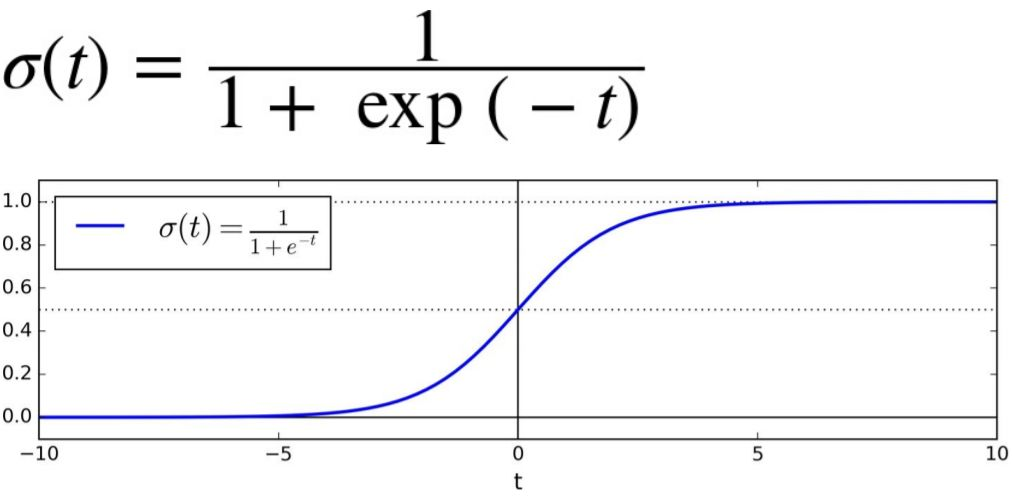
\includegraphics[width=0.4\linewidth]{imgs/sigmoide}
    \caption{Sigmoide}
    \label{fig:sigmoide}
\end{figure}

\subsubsection{Funzione logistica}
La regressione logistica calcola dei pesi per gli input + un termine bias.

Si si devono attribuire più label, si utilizzano tante classificazioni binarie.

\subsection{Classificazione multi-classe}
\subsubsection{One vs All}
Vengono allenate tante logistc classifier(binary), un classificatore per
ogni classe, poi si classifica in base alla probabilità dell oggetto per ogni classe.



\subsection{Dare un voto alle task di calssificazione}
\begin{itemize}
    \item matrice di confusione
    \item accuratezza
    \item precisione
    \item recall
    \item F-1
    \item curva di ROC
\end{itemize}

\subsubsection{Matrice di confusione}


\begin{figure}[H]
    \centering
    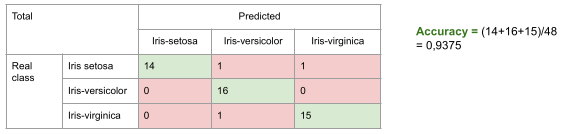
\includegraphics[width=0.5\linewidth]{imgs/matrice-di-confusione}
    \caption{matrice di confusione}
    \label{fig:conf_matrix}
\end{figure}

\subsubsection{Accuratezza}
Rapporto tra le predizioni corrette sul totale delle predizioni.(spesso si usa
la percentuale)


\textbf{Se il test set non è bilanciato, questo valore non ha nessun senso utile.}

\subsubsection{dataset non bilanciato}
Se il dataset non è bilanciato non devo vedere quante volte ci prendo sul totale
ma quante volte ci prendo sulla classe in analisi.

\subsubsection{Precisione}
Come l'accuratezza delle predizioni positive.

\begin{figure}[H]
    \centering
    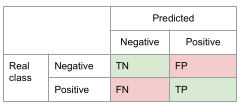
\includegraphics[width=0.2\linewidth]{imgs/precisione}
    \caption{Precisione}
    \label{fig:precisione}
\end{figure}


\begin{equation}
    Precisione = \frac{TP}{TP+FP}
\end{equation}


\subsubsection{Recall}
Conosciuta anceh come sensibilità o rateo di veri positivi.

È il rapporto di istanze positive che vengono correttamente trovate
dal classificatore.

\begin{equation}
    Recall = \frac{TP}{TP+FN}
\end{equation}

\subsubsection{F-1}
Misura armonica di precisione e recall,
tratta tutti i valori in maniera uguale,
attribuendo maggiore importanza ai valori bassi.

Un F1 alto è caratterizzato sia da recall alto che da precision alto!


\begin{equation}
    F_1 = \frac{2}
    {\frac{1}{Precision} +
    \frac{1}{Recall}}
\end{equation}


\subsubsection{Decision tree}
Modello ML simile ad un flowchart, le foglie sono le
classi(usabile sia in regression che classification).

Nel decision tree si usa il GINI.
\begin{equation}
    G_i = 1 - \sum_{k=1}^{n}p_{i,k}^2
\end{equation}

Si cerca d iscendere fino ad avere un gini = 0.

\subsubsection{CART}
CART(Classification and Regression Tree algorithm)
\begin{enumerate}
    \item dividi il training in 2 subsets usando una features k e una trashold $t_k$
    \item per prendere k e $t_k$ ci si basa sul subset più puro
    \item si ferma quando si raggiunge la profondità massima
\end{enumerate}

\begin{figure}[H]
    \centering
    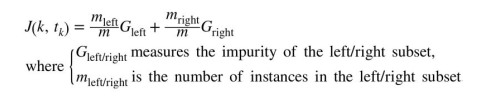
\includegraphics[width=0.7\linewidth]{imgs/cart}
    \caption{CART}
    \label{fig:CART}
\end{figure}

\subsubsection{Gini VS Entropia}
In ML, l'entropia è zero solo se l'istanza contiene una classe.

\begin{equation}
    H_i = - \sum_{k=1, P_{i,k}\neq 0}^{n}
    p_{i,k}\log(p_{i,k})
\end{equation}

Non ci sono tante differenze fra gini e entropia, solo che il gini essendo una sommatoria
è più veloce da calcolare e tende ad isolare la classe più frequente,
mentre l'entropia produce alberi più bilanciati.

\subsubsection{Regressione con alberi decisionali}
L'algoritmo splitta a scalini il tutto in mod oda avere tante istanze
di training vicine al possibile valore:
\begin{figure}[H]
    \centering
    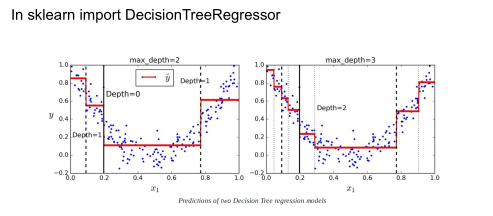
\includegraphics[width=0.5\linewidth]{imgs/decisiontreeregressor}
    \caption{DecisionTreeRegressor}
    \label{fig:DecisionTreeRegressor}
\end{figure}


Il CART funziona come prima però non cerca di splittare il
training set ma di minimizzare le impurità.

\subsubsection{Problemi: overfitting}
\begin{itemize}
    \item i decison tree fanno meno assunzioni rispetto al modello lineare
    \item se lasciato senza vincoli, va SUPER in over fitting
    \item l'albero è più libero come parametri, mentre la regressione lineare è
    più vincolata
\end{itemize}

\subsubsection{Soluzione: regolarizzazione}
Una soluzione è risurre i gradi di liberta dell'albero durante la fase di
training(regolarizzazione).
\begin{itemize}
    \item massima profondità
    \item numero minimo di campionimassimo numero di features per dividere i nodi
\end{itemize}

Metodologia del \textbf{pruning}, prima si fa il modello senza vincoli e poi si
applicano vincoli in base al caso.



Sensibili alla rotazione della matrice dei dati.